
\subsubsection{Parameter Estimates}
\label{subsec : param_estimates_jm_fit_prias}
The posterior parameter estimates for the joint model we fitted to the PRIAS dataset are shown in Table \ref{tab : PSA_long} and Table \ref{tab : PSA_survival}. Since the longitudinal evolution of $\log_2 \mbox{PSA}$ is modeled with non-linear terms, the interpretation of the coefficients corresponding to time is not straightforward. In lieu of the interpretation we present the fitted evolution of PSA (Figure \ref{fig : fitted_trend_psa}) over a period of 10 years for a patient who is 70 years old. It can be seen that after the first 6 months the PSA levels steadily increase over the follow up period. Since the model for PSA has only additive terms, this evolution remains same for all patients. The effect of age only affects the baseline PSA score. However it is so small that it can be ignored for all practical purposes.

For the relative risk sub-model, the parameter estimates in Table \ref{tab : PSA_survival} show that only $\log_2 \mbox{PSA}$ velocity is strongly associated with hazard of GR. For any patient, a unit increase in $\log_2 \mbox{PSA}$ velocity corresponds to a 11 time increase in hazard of GR. The effect of $\log_2 \mbox{PSA}$ value and effect of Age on hazard of GR are small enough to be safely ignored for all practical purposes.

\begin{figure}
\centerline{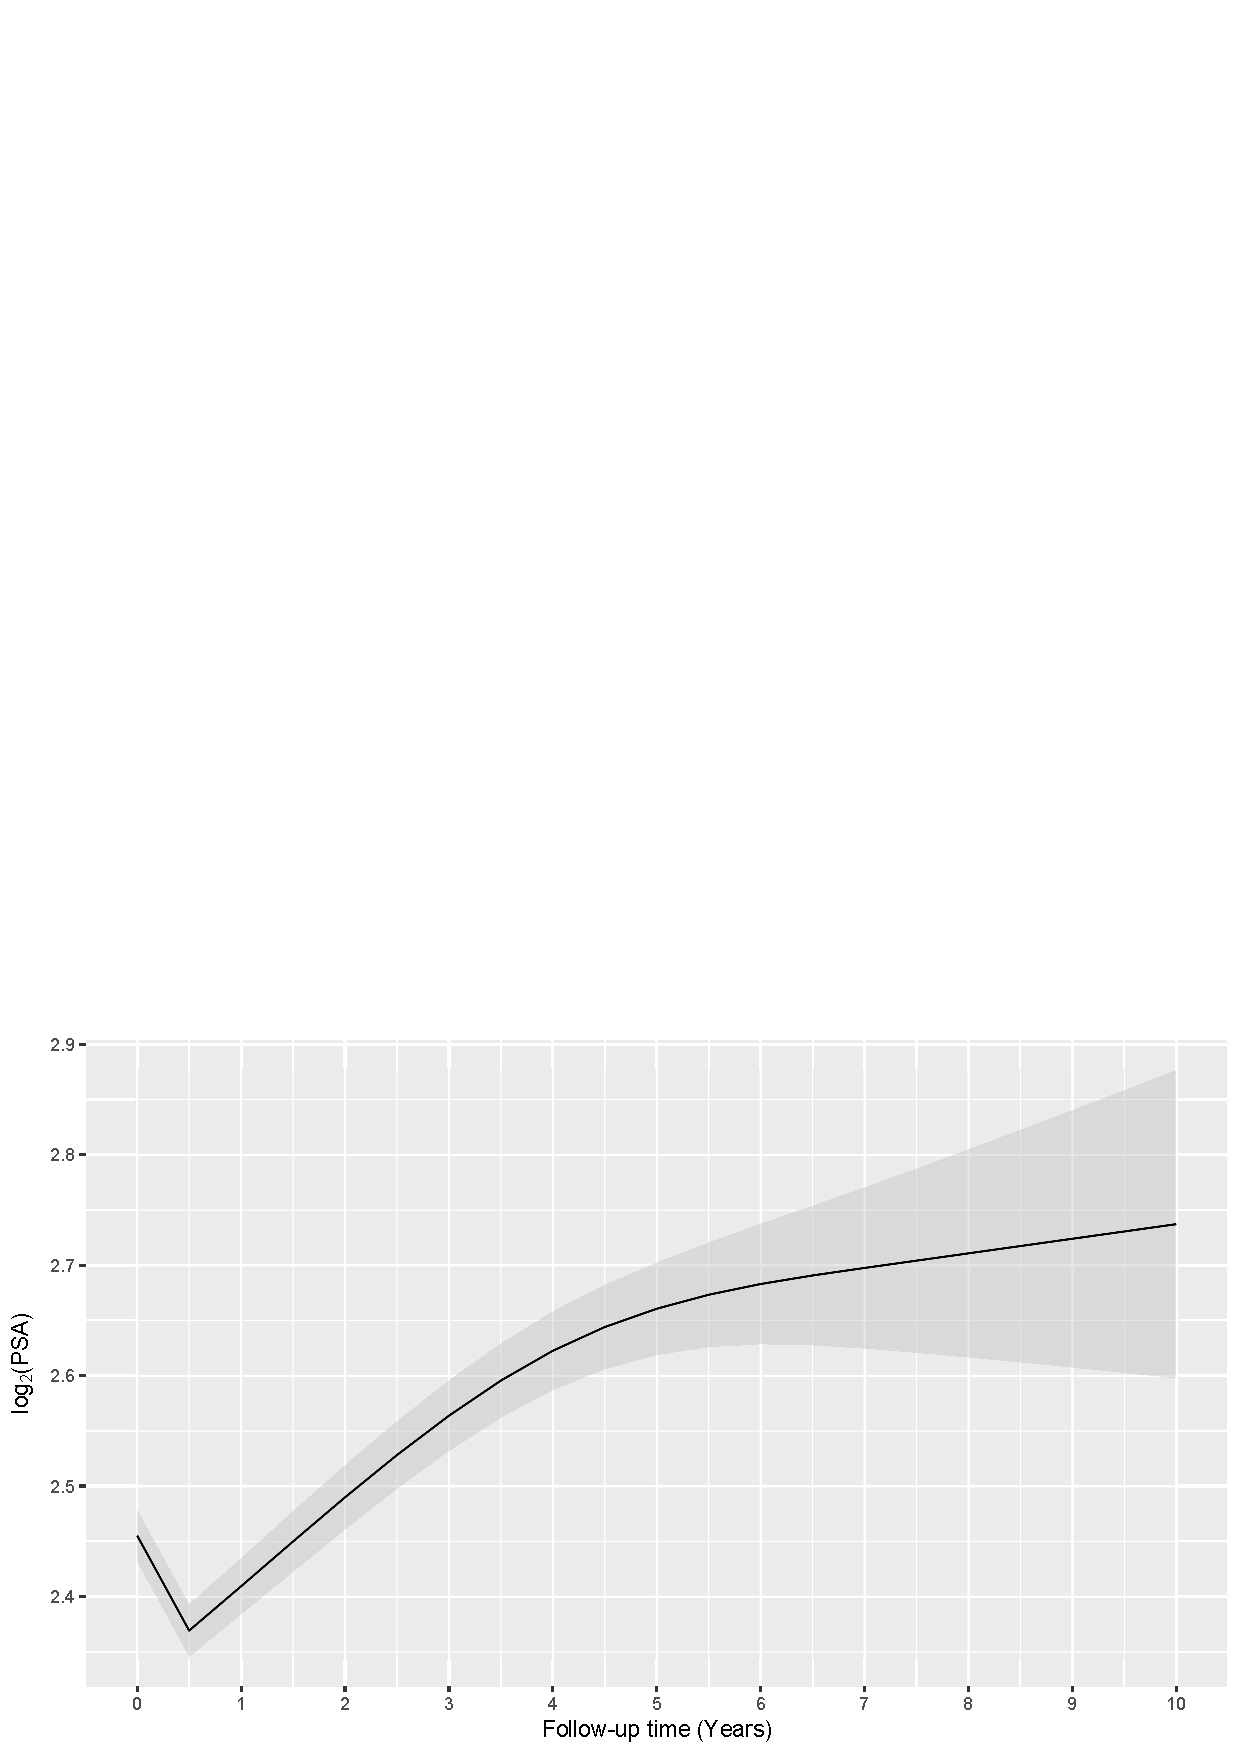
\includegraphics[width=\columnwidth]{images/fitted_trend_psa.png}}
\caption{Fitted evolution of $\log_2 \mbox{PSA}$ over a period of 10 years, for a patient who was inducted in AS at the Age of 70 years.}
\label{fig : fitted_trend_psa}
\end{figure}

\begin{table}
\caption{Longitudinal sub-model estimates for joint model.}
\label{tab : PSA_long}
\begin{tabular}{lrrrrr}
\Hline
& Mean   & Std. Dev           & 2.5\%               & 97.5\%              & P              \\ \hline
Intercept                            &  2.455 & 0.012 & 2.433 & 2.480               & \textless0.000 \\
(Age - 70)                           & 0.003 & 0.001 & 4.9 $\times 10^{-4}$ & 0.006 & 0.032          \\
(Age - 70) $\times$ (Age - 70)       & -0.001 & 1.4 $\times 10^{-4}$ & -0.001 & -3.5 $\times 10^{-4}$ & \textless0.000 \\
Spline: visitTimeYears{[}0, 0.5{]}   & -0.006 & 0.012 & -0.031 & 0.017 & 0.674 \\
Spline: visitTimeYears{[}0.5, 1.2{]} & 0.228 & 0.019 & 0.192 & 0.265               & \textless0.000 \\
Spline: visitTimeYears{[}1.2, 2.5{]} & 0.140 & 0.029 & 0.088 & 0.197               & \textless0.000 \\
Spline: visitTimeYears{[}2.5, 7{]}   & 0.303 & 0.039 & 0.227 & 0.379               & \textless0.000 \\
$\sigma$                               & 0.324 & 0.001 & 0.321 & 0.326              &  \\ \hline
\end{tabular}
\end{table}

\begin{table}
\caption{Survival sub-model estimates for joint model.}
\label{tab : PSA_survival}
\begin{tabular}{lrrrrr}
\Hline
Variable                      & Mean   & Std. Dev & 2.5\%  & 97.5\%                 & P              \\ \hline
Age - 70                      & 0.037 & 0.006 & 0.025 & 0.0490                  & \textless0.000 \\
(Age - 70) $\times$ (Age - 70) & -0.001 & 0.001 & -0.003 & 1.8 $\times 10^{-4}$ & 0.104          \\
$\log_2 \mbox{PSA}$                  & -0.049 & 0.064 & -0.172 & 0.078 & 0.414         \\
Slope($\log_2 \mbox{PSA}$)           & 2.407 & 0.319 & 1.791 & 3.069 & \textless0.000 \\
\hline
\end{tabular}
\end{table}